\documentclass[11pt,letterpaper]{article}
\pdfvariable minorversion=7
\usepackage[left=0.91in,right=0.91in,top=0.92in,bottom=0.95in,headheight=14pt,headsep=15pt]{geometry}
\usepackage{fontspec}
\usepackage{libertinus}
\usepackage{microtype,graphicx,amsmath,array,booktabs,xltabular}
\usepackage{caption}
\usepackage[section]{placeins}
\usepackage{titlesec,enumitem,fancyhdr,needspace}
\usepackage[dvipsnames]{xcolor}
\definecolor{ink}{HTML}{253044}
\definecolor{accent}{HTML}{43537C}
\usepackage[unicode,colorlinks=true,urlcolor=accent,linkcolor=accent]{hyperref}
\hypersetup{pdftitle={From Fragmented Evidence to Analyzable Biomedical Cohorts with Scientific Agents}, pdfauthor={}}
\setcounter{secnumdepth}{2}
\titleformat{\section}{\sffamily\Large\bfseries\color{ink}}{\thesection}{.65em}{}
\titleformat{\subsection}{\sffamily\large\bfseries\color{ink}}{\thesubsection}{.65em}{}
\titlespacing*{\section}{0pt}{2.2ex plus .4ex minus .1ex}{.9ex}
\titlespacing*{\subsection}{0pt}{1.7ex plus .3ex minus .1ex}{.6ex}
\captionsetup{font=small,labelfont={bf,color=ink},labelsep=period,justification=raggedright,singlelinecheck=false}
\setlength{\parindent}{0pt}
\setlength{\parskip}{.45em plus .08em minus .03em}
\setlength{\LTpre}{.9em}
\setlength{\LTpost}{.9em}
\setlength{\LTcapwidth}{\textwidth}
\setlength{\textfloatsep}{16pt plus 4pt minus 2pt}
\setlength{\intextsep}{12pt plus 3pt minus 1pt}
\setcounter{topnumber}{3}
\renewcommand\topfraction{.85}
\renewcommand\bottomfraction{.7}
\renewcommand\textfraction{.12}
\renewcommand\floatpagefraction{.68}
\renewenvironment{abstract}{\small\par\noindent{\sffamily\bfseries\color{ink}Abstract}\quad\ignorespaces}{\par\medskip}
\pagestyle{fancy}
\fancyhf{}
\fancyhead[L]{\small\sffamily\color{accent}Evidence-guided virtual cohorts}
\fancyhead[R]{\small\sffamily\color{accent}Methods development draft}
\fancyfoot[R]{\small\sffamily\thepage}
\renewcommand\headrulewidth{0.25pt}
\raggedbottom
\clubpenalty=10000
\widowpenalty=10000
\emergencystretch=3em
\begin{document}
\thispagestyle{plain}
{\sffamily\footnotesize\color{accent}\bfseries METHODS DEVELOPMENT DRAFT\quad\textbar\quad 17 NOVEMBER 2026\par}
\vspace{.7em}
{\raggedright\sffamily\bfseries\fontsize{24}{29}\selectfont\color{ink}From Fragmented Evidence to Analyzable Biomedical Cohorts with Scientific Agents\par}
\vspace{.5em}
{\small Author and affiliation details pending confirmation\par}
\vspace{.7em}
\begin{abstract}

Published biomedical findings are available even when the individual measurements needed for a new analysis are not. We study how scientific Agents can turn a research request and fragmented evidence into virtual cohorts that existing analysis software can use. The Agent interprets study conditions, combines compatible statistics, chooses a joint probability model and authors an executable generator. Numerical tools sample the model, check its outputs and preserve a source-to-assumption record. We evaluate scientific use through the same analyses on virtual and measured records, rather than marginal similarity alone. A lifestyle application reproduces an adjusted urban–\allowbreak{}pastoralist BMI contrast of 1.700–\allowbreak{}2.251 kg/\allowbreak{}m² across six generated cohorts, compared with 1.882 in the measured sample. Two controlled tasks show composition of complementary evidence into adjusted and within-person relationships. Two biomedical three-condition experiments then separate the addition of marginal summaries from the addition of joint statistics. Relative to summaries alone, joint evidence reduces residual-correlation discrepancy by 78.6\% in blood pressure and absolute log-odds-ratio discrepancy by 46.8\% in iron status. The complete profiles also reveal unchanged or worsened slopes, prevalence and continuous dependence. The contribution is an analysis-driven, inspectable route from evidence to records, with concrete evidence that joint information can improve a requested scientific use. These developmental results delimit the supported analyses; they do not establish clinical equivalence or general transport to new populations.

\end{abstract}

\Needspace{8\baselineskip}

\section{Introduction}

Biomedical researchers often know the measurements and analyses a study needs before they can obtain a complete dataset. A cohort may omit an expensive biomarker, individual records may be inaccessible, or the available knowledge may consist only of papers describing different parts of a joint relationship. Published means, adjusted coefficients and subgroup counts are valuable, but cannot simply be concatenated into patient records. The practical opportunity is to make that evidence usable through a virtual data product.


Consider two requests. One asks for paired blood-pressure measurements suitable for an age-, sex- and BMI-adjusted analysis. Another asks for hemoglobin and ferritin measurements suitable for both deficiency co-occurrence and continuous association analysis. A collection of marginal summaries is insufficient for either joint task. Even a published correlation may describe a different adjustment set. The generator must supply a coherent joint law, including explicit choices where evidence is missing.


We study scientific Agents as model authors in this setting. Given a population, measurements, intended analyses and permitted evidence, an Agent interprets the sources, selects or derives constraints, chooses the scientific structure and writes a sampler. The resulting records can be passed to ordinary regression, group-comparison and joint-association software. The method includes complete cohort generation with no target individual input. Extending unmeasured columns and completing partially missing records are related uses with different information boundaries; they require separate validation.


The central scientific question is not answered by a plausible table alone: \textbf{which analyses can the generated data support, and what changes when the evidence covers the joint relationship those analyses require?} Generating more rows reduces sampling noise under a chosen law. Supplying complementary relationship evidence can change that law. Our experiments distinguish these two operations and show both the useful consequences and their limits.


We make three contributions. \textbf{First, an executable task and workflow:} a scientific request is translated into a joint model, virtual records and a traceable evidence/\allowbreak{}assumption record, with Agent decisions separated from deterministic execution. \textbf{Second, evidence-composition experiments:} two controlled tasks test mathematical composition, followed by two biomedical content controls that isolate the addition of joint statistics beyond marginal summaries. \textbf{Third, analysis-level evaluation:} the same scientific estimators are applied to virtual and measured records, with complete endpoint profiles and worked model-choice traces. The strongest experimental finding is a specific improvement in two requested joint analyses, not a universal quality gain across every use of a table.


\Needspace{8\baselineskip}

\section{Related work and task position}

LLM-based simulation and summary-driven synthesis already cover important parts of this space. G-Sim proposes simulator structure and calibrates it with gradient-free optimization or simulation-based inference [1]. LLMSynthor uses aggregate alignment, inferred dependencies and statistical differences to guide synthetic records [2]. Biomedical approaches include simulation from summary rules for data pooling [3], SynthIPD's reconstruction from published materials [4], KMGen's literature-informed patient generation [5] and SynthCraft's medical synthetic-data workflow [6]. Agent terminology, a sampling program or a feedback loop alone does not distinguish the present work.


Our emphasis is the scientific modeling task connecting a biomedical request to the joint relationships needed for its analysis. We make the adopted study conditions and unsupported completions inspectable, and test what an increment of joint evidence changes in the delivered data. The biomedical examples cover adjusted pressure dependence and threshold-versus-continuous biomarker association, alongside a lifestyle reconstruction. We do not establish quality superiority over the neighboring systems; matched tasks and comparable inputs would be needed for that claim.


Statistical integration is an essential foundation. Multilevel network meta-regression relates individual models to study-level evidence [7], and SynDI incorporates external models through synthetic data [8]. Covariance projection, copulas and summary matching are established statistical tools. The Agent contribution is to interpret the evidence and construct a suitable executable combination for a request. Whether that construction is useful in a target sample remains an empirical question, separate from correctly executing the statistical algebra.


\Needspace{8\baselineskip}

\section{Method: from a research request to an executable joint model}

\FloatBarrier

\Needspace{5\baselineskip}

\subsection{Define the requested data and analyses}

A request specifies the target population, measurement definitions and units, desired record structure, planned analyses and available inputs. It may supply no individual measurements, permitted covariates, or partially observed records. The main experiments here generate complete fictional records without target individual inputs. The request may explicitly name an intended analysis; it need not hide the user's scientific question. Evaluation measurements and results are withheld from fresh constructor contexts.


The output is more than a CSV: it includes the Agent-authored program, a model specification, parameter origins and the generated records. A new user request may legitimately lead to a different model. Freezing a delivery fixes one evaluation boundary; it does not force all future requests to use one immutable generator.


\begin{figure}[htbp]

\centering

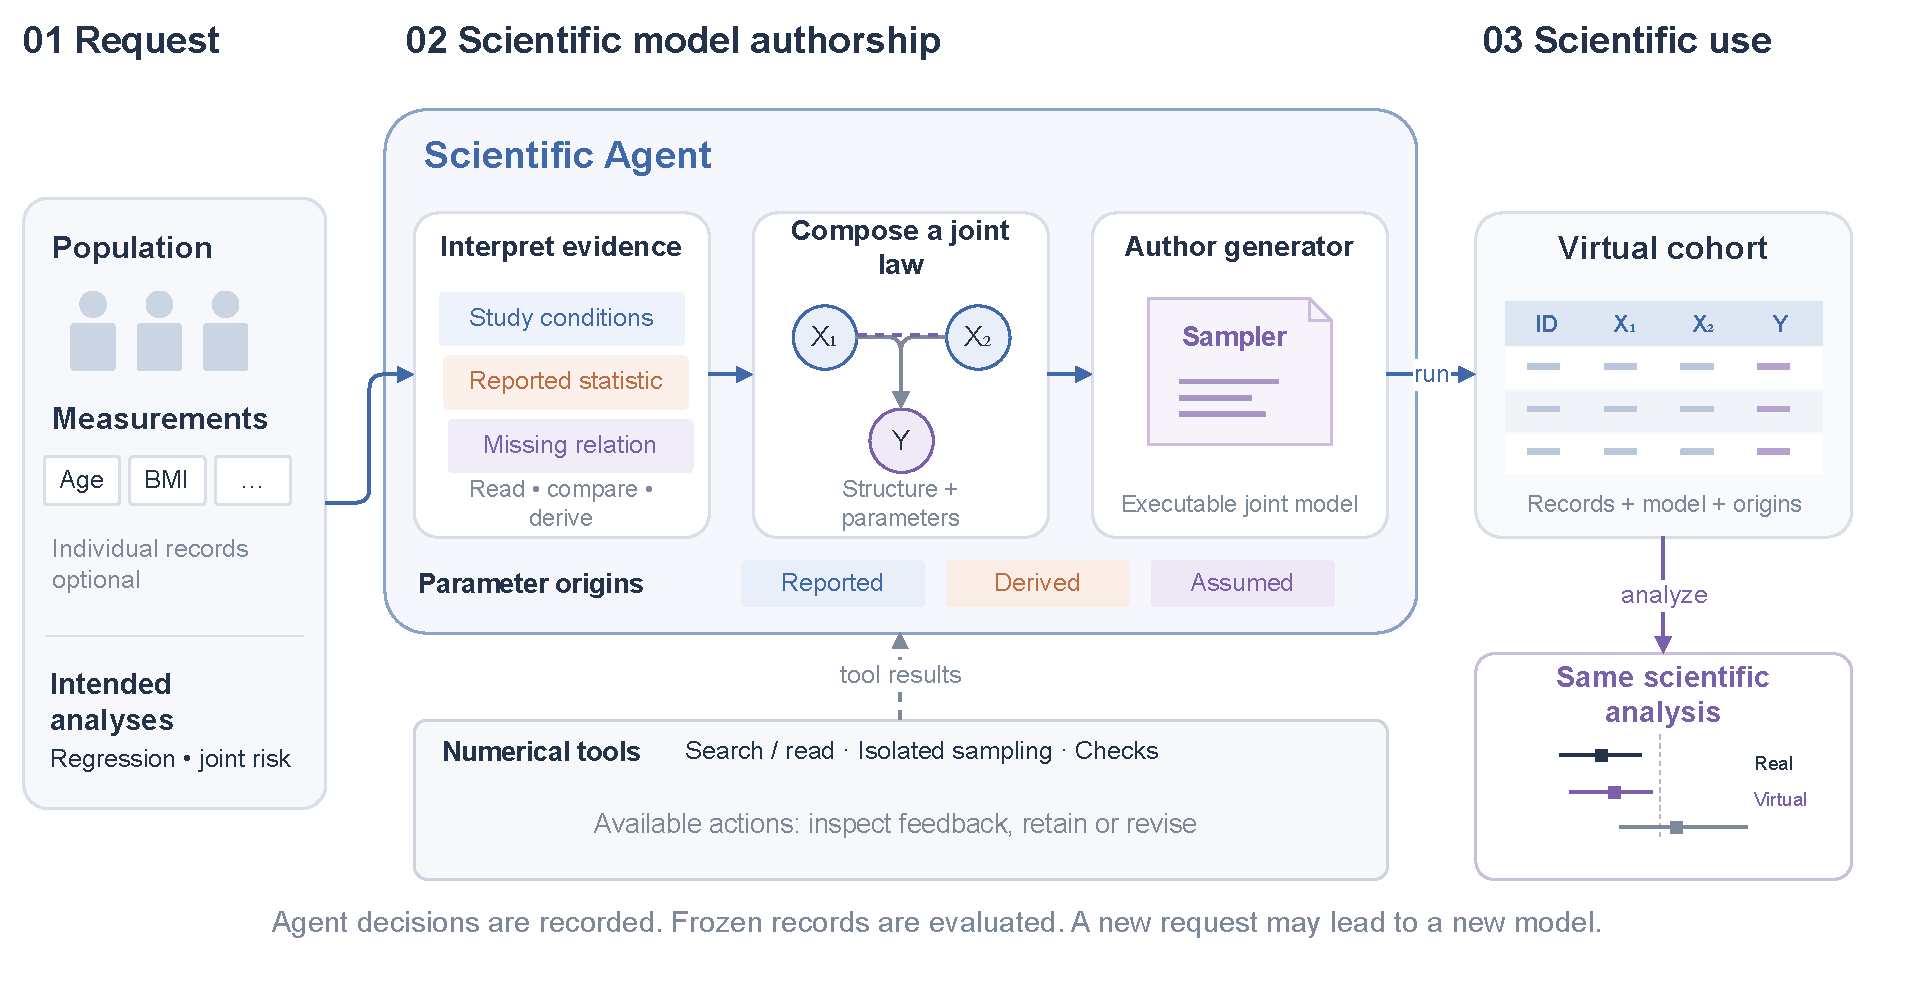
\includegraphics[width=\linewidth]{figures/fig1-request-to-data.drawio.pdf}

\caption{The Agent authors the scientific model; tools produce and inspect its records. The Agent reads study conditions, composes supported relationships, selects a joint law and writes the generator. Numerical tools execute that law in isolation. The delivered table is analyzed with the same estimator used for its measured-sample comparison. The origin record links adopted parameters to reported evidence, derivations and remaining assumptions. Search and diagnostic revision are available actions; the new content-control experiments use fixed evidence packets and one construction call to isolate information content. Their evidence admission includes coordinator review, not fully automated source certification. The small table and analysis marks are schematic, not experimental observations.}

\label{fig:1}

\end{figure}

\FloatBarrier

\Needspace{5\baselineskip}

\subsection{Interpret evidence under its study conditions}

Each evidence item retains its original population, measurement, unit, transformation, statistic, adjustment set and available uncertainty. A marginal Pearson correlation, a Spearman correlation and an adjusted residual correlation are different constraints. Source summaries also require compatible observations: covariances cannot be reconstructed from variances measured in unrelated subsets without further assumptions.


When retrieval is allowed, the Agent can search for missing information and inspect original material. The completed blood-pressure search used Europe PMC queries and retrieved full texts. A coordinating research assistant then checked methods and tables and withheld an ambiguous candidate. In the content-control experiments, the coordinator instead supplied audited, masked source packets. This separates an actual retrieval episode from a controlled test of what information a constructor receives.


Each consequential model choice is marked as reported, derived or assumed. These are composable descriptions of origin, not ranked confidence levels. A source residual correlation can be derived correctly while its transfer to a new population remains assumed. We preserve five distinct quantities: the published statistic, the adopted parameter, the complete model's implied analysis, the estimate from sampled records and the measured-sample comparator. Their separation makes a modeling decision inspectable without treating a provenance label as an accuracy certificate.


\FloatBarrier

\Needspace{5\baselineskip}

\subsection{Let the Agent construct the joint law}

The Agent chooses distributions, dependence structure, numerical parameters and how to complete underidentified relationships. It then authors the executable sampler. The host supplies an interface and the permitted inputs, not the desired target slope, correlation, odds ratio or expected sign. The main implementation is therefore Agent-authored programmatic generation: numerical software samples the scientific law that the Agent wrote. It is not direct token-by-token generation of every patient row.


This freedom has observable consequences. In the pressure experiment, Agents derive residual covariance from a reported matrix and select an innovation law and transfer assumption. In the iron experiment, Agents choose a copula and solve for a latent dependence parameter from four published cells. In the repeated-measure task, they separate stable person components from visit deviations. These are case-specific constructions; neither a fixed copula nor a fixed regression is the overall method.


When the evidence does not identify the requested relationship, a scenario can still be delivered with its assumptions recorded. Several source-consistent laws may support different downstream analyses. Repeated seeds explore sampling under one law; they do not express uncertainty across those unreported scientific possibilities.


\FloatBarrier

\Needspace{5\baselineskip}

\subsection{Execute, check and close the delivery}

The submitted programs run through an isolated worker, using WSL/\allowbreak{}bubblewrap with a cleared environment, unshared network, read-only code/\allowbreak{}runtime inputs and bounded resources. Schema, row counts, finite outputs and hashes are checked outside the Agent. Mathematical review examines support and relevant moments; physiological review examines measurement-consistent restrictions; scientific checks compare estimable source relationships. A source check is unavailable when its statistical operator or population conditions cannot be reproduced. Unavailable checks are not counted as passes.


The broader workflow can return permitted diagnostics to the Agent for a keep-or-revise decision. The two new content controls deliberately use one call per construction, without retries, feedback or host scientific repairs. This design tests evidence content and the Agent's initial model construction, not revision benefit. Programs and specifications close before all final tables are analyzed. Every planned construction and draw is retained.


API records retain requested and returned model identifiers, prompts, outputs, tool interactions, usage and tariff-based cost estimates. Program replay and model-decision reproducibility are different: the same scientific program can be resampled, whereas a new stochastic API session may choose another law.


\FloatBarrier

\Needspace{5\baselineskip}

\subsection{Measure usefulness through scientific analyses}

We apply the same analysis implementation to virtual and reference records, with the weighting appropriate to each design. Outcomes include adjusted contrasts, BMI slopes, linear-residual correlation, deficiency odds ratios, joint prevalence and rank correlation. For each construction, estimates from its prespecified seeds are averaged; construction-level summaries then receive equal weight. Discrepancies are calculated at the draw level before this averaging. This prevents an average across opposing errors from masquerading as accurate generation.


Measured samples provide uncertain references, not known population truths. Reference confidence intervals describe their own sampling design and are not automatic acceptance margins. Likewise, virtual draw ranges are Monte Carlo variation, not clinical-effect intervals. Controlled mathematical tasks have prespecified numerical tolerances. Biomedical adequacy is reported in analysis units; no retrospective equivalence threshold or universal quality score is introduced.


\Needspace{8\baselineskip}

\section{Evaluation design}

\FloatBarrier

\begingroup

\small

\renewcommand{\arraystretch}{1.22}

\begin{xltabular}{\linewidth}{@{}>{\raggedright\arraybackslash}X>{\raggedright\arraybackslash}X>{\raggedright\arraybackslash}X>{\raggedright\arraybackslash}X@{}}

\caption{Four main study blocks test different parts of the evidence-to-data claim. Seeds are nested within constructions.}\label{tab:1} \\

\toprule

\textbf{Study and scientific use} & \textbf{Information available to the Agent} & \textbf{Construction scale} & \textbf{Evaluation role} \\

\midrule

\endfirsthead

\multicolumn{4}{l}{\small Table \thetable\ continued}\\

\toprule

\textbf{Study and scientific use} & \textbf{Information available to the Agent} & \textbf{Construction scale} & \textbf{Evaluation role} \\

\midrule

\endhead

\bottomrule

\endfoot

Lifestyle: adjusted group contrasts & Original paper, group findings and context; no target individual records & 2 constructions; 6 tables of 1,226 & Source-rich reconstruction of a real analysis \\

Controlled composition: adjusted and within-person association & Basic summaries, A, B, or A+B; stipulated artificial structure & 24 constructions; 72 tables of 3,000 & Algebraic composition and underidentification \\

Blood pressure: slopes and residual dependence & BASE, +SUMMARY, or +JOINT from one added paper & 9 constructions; 27 tables of 3,000 & Developmental evidence-content comparison \\

Iron status: threshold and continuous association & Study context, +SUMMARY, or +JOINT from one paper & 9 constructions; 27 tables of 5,000 & Second developmental content comparison \\

\end{xltabular}

\endgroup

\FloatBarrier

\Needspace{5\baselineskip}

\subsection{A real analysis with the data replaced}

Lea et al. studied cardiometabolic variation across pastoralist, rural and urban Turkana lifestyles [9]. Two fresh Agent authors generated age, sex, lifestyle, BMI, total cholesterol and HDL cholesterol. The measured analytical pool comprised 1,226 eligible adults, with BMI, total cholesterol and HDL available for 1,189, 400 and 405 participants, respectively. Each virtual table contained all measurements for 1,226 fictional individuals.


We reimplemented the analysis from the published Methods and applied the same implementation to both data types. Original author software was unavailable; this is not an unchanged run of their code or replication of every paper result. All nine pooled adjusted pairwise lifestyle contrasts are primary. Sex-specific contrasts, interaction tests and diagnostics remain available. Because the original published group findings were permitted inputs, this is reconstruction, not independent discovery.


\FloatBarrier

\Needspace{5\baselineskip}

\subsection{Complementary evidence in two controlled tasks}

The first artificial task requests the correlation of X and Y after separate linear adjustment for Z. Basic records give standardized marginal moments; A gives the X–\allowbreak{}Y correlation; B gives both correlations with Z. Together they identify a residual correlation of 0.21875. The second task requests the correlation of two biomarkers' within-person changes. Its stipulated structure separates stable person components from independent visit deviations. A gives between-person correlation and B same-visit correlation; together they identify change correlation −0.6. Supplement S2 states the exact assumptions and derivations.


Each task has four information conditions and three fresh constructions per cell. There are 24 first attempts and 72 draws, without retries or repair calls. The numerical tolerance for identified correlations and slopes is 0.08; separate source diagnostics use the frozen scale-specific rules. These are mathematical implementation tolerances, not clinical equivalence margins. In incomplete conditions the primary relationship is underidentified, so we show the selected scenarios without grading them against one hidden completion.


\FloatBarrier

\Needspace{5\baselineskip}

\subsection{Two biomedical evidence-content controls}

The blood-pressure experiment uses an existing PNS analysis for adults aged 20–\allowbreak{}79 [10]. Its three primary quantities are both BMI–\allowbreak{}pressure slopes and residual SBP–\allowbreak{}DBP Pearson correlation. The common design matrix contains intercept, age per decade centered at 50, female indicator and BMI per 5 kg/\allowbreak{}m² centered at 25. Both pressure SDs and physiological ordering are diagnostics. The existing weighted complete-case laboratory-substudy analysis is the comparator; generated rows are equally weighted draws of the proposed analytical population.


The iron experiment uses an existing NHANES August 2021–\allowbreak{}2023 reference [14] for 979 nonpregnant women aged 20–\allowbreak{}44 with both measurements and positive phlebotomy weights, without a CRP restriction. Its primary analyses are crude association of low Hb and low ferritin, their joint prevalence and continuous Spearman correlation. Thresholds are strictly Hb <12 g/\allowbreak{}dL and ferritin <15 μg/\allowbreak{}L. Single-marker prevalences are diagnostics. Source evidence comes from Zhu et al.'s study of 1,671 selected rural Chinese women [13].


\FloatBarrier

\Needspace{18\baselineskip}

\FloatBarrier

\begingroup

\small

\renewcommand{\arraystretch}{1.22}

\begin{xltabular}{\linewidth}{@{}>{\raggedright\arraybackslash}X>{\raggedright\arraybackslash}X>{\raggedright\arraybackslash}X>{\raggedright\arraybackslash}X@{}}

\caption{Within-case information masks. JOINT versus SUMMARY is the primary content comparison; BASE has a different meaning in the two cases.}\label{tab:2} \\

\toprule

\textbf{Case} & \textbf{BASE} & \textbf{Added in SUMMARY} & \textbf{Added only in JOINT} \\

\midrule

\endfirsthead

\multicolumn{4}{l}{\small Table \thetable\ continued}\\

\toprule

\textbf{Case} & \textbf{BASE} & \textbf{Added in SUMMARY} & \textbf{Added only in JOINT} \\

\midrule

\endhead

\bottomrule

\endfoot

Blood pressure & Existing packet, including INTERSALT coefficients and a raw-covariance source & Burkina Faso study context and univariate summaries [11] & Six same-sample pairwise correlations \\

Iron status & Zhu study identity, population and measurements, without selected outcome statistics & Low-marker counts and ferritin geometric mean & Four paired threshold cells from the same women \\

\end{xltabular}

\endgroup

Within each case all arms use the same request, model and construction interface. SUMMARY and JOINT contain the same marginal evidence; only JOINT receives the paired block. Packets contain the reported values, not a host-derived target dependence parameter. Iron BASE is not the earlier full iron packet, and PNS BASE already contains some relationship information. These are not interchangeable no-evidence controls.


Each experiment uses nine fresh \texttt{gpt-\allowbreak{}6.1-\allowbreak{}sol} constructions with high reasoning and default service, shuffled once before calls: three per arm, one call each, three fixed seeds per program. All 18 constructions and 54 final tables completed. Constructors did not see reference outcomes, old programs or prior results. Both references were already exposed to the project; PNS was selected following a favorable two-arm follow-up. These are frozen developmental comparisons, not two unseen-population validations. No patient refit or new data download was needed.


For PNS the primary contrast is absolute residual-correlation discrepancy. For iron it is absolute natural-log OR discrepancy. Both are averaged within constructions and then across constructions. All other prespecified endpoints are co-reported. No pooled cross-case score, significance claim or row-based effective sample size is used.


\Needspace{8\baselineskip}

\section{Results}

\FloatBarrier

\Needspace{5\baselineskip}

\subsection{Virtual records support a concrete lifestyle analysis}

The generated cohorts reproduce a clear urban BMI contrast. Across six draws, urban-minus-pastoralist BMI is 1.700–\allowbreak{}2.251 kg/\allowbreak{}m², against 1.882 in the measured sample (95\% model-based interval 1.368–\allowbreak{}2.397). The same table format supports all planned adjusted comparisons without a custom analyzer for each generator. Figure 2 shows the full nine-contrast profile.


Other findings are less well represented. Urban-minus-pastoralist total cholesterol is 13.732–\allowbreak{}18.907 mg/\allowbreak{}dL against 20.342, while rural lipid contrasts and HDL contrasts can differ in direction. Total-cholesterol SD is approximately 31.85–\allowbreak{}34.06 versus 42.81 mg/\allowbreak{}dL; HDL SD is approximately 14.4–\allowbreak{}15.1 versus 20.23. Standardization can obscure such scale differences, so the figure uses original units. Supplement S1 preserves complete estimates and auxiliary checks.


\begin{figure}[htbp]

\centering

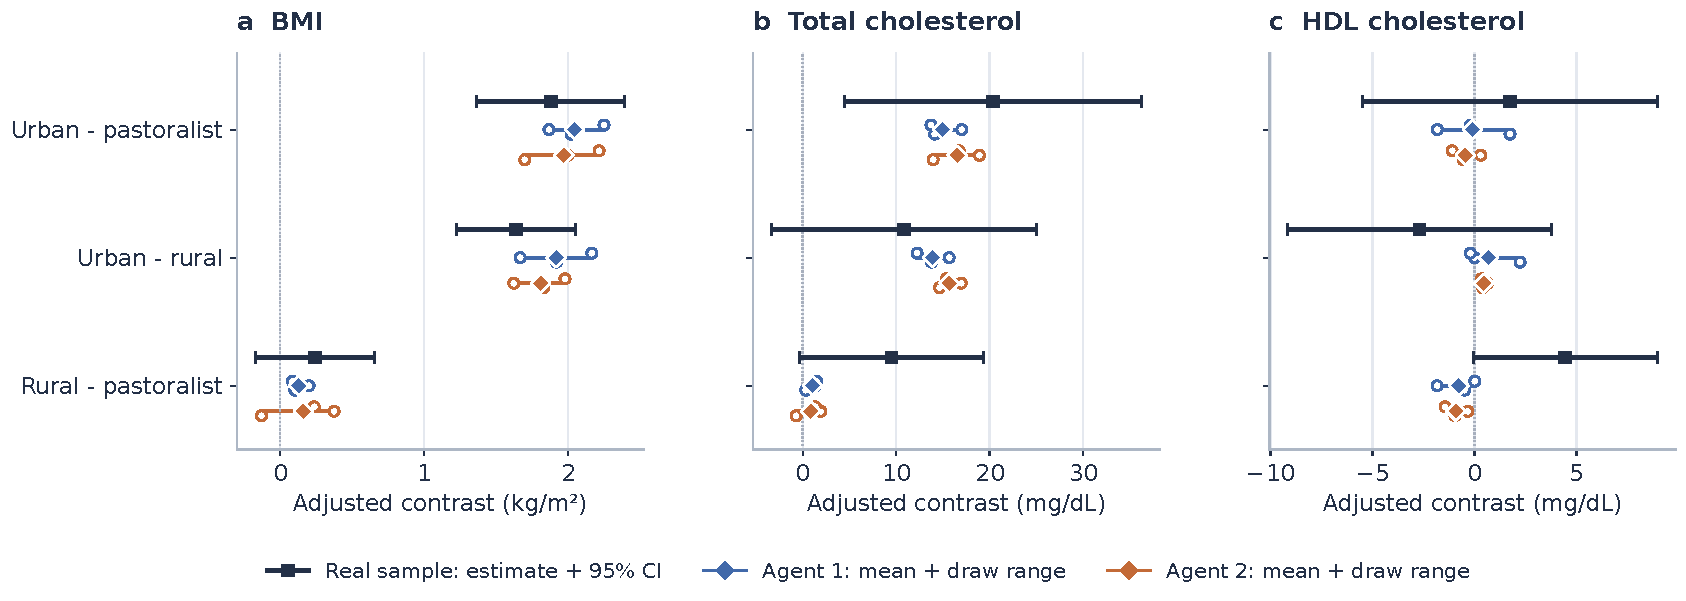
\includegraphics[width=\linewidth]{figures/fig2-scientific-use.pdf}

\caption{Replace the data, retain the analysis. Dark squares and bars are measured-sample estimates and model-based 95\% intervals. Colored diamonds are the means of three draws from each Agent construction; open circles and ranges are those draws. All nine pooled adjusted contrasts are shown in original units. The BMI contrasts are well represented in this reconstruction; lipid contrasts show remaining differences. Published findings were allowed inputs. Reference measurement availability differs by biomarker, whereas virtual records are complete.}

\label{fig:2}

\end{figure}

\FloatBarrier

\Needspace{5\baselineskip}

\subsection{Agents compose information into relationships that are not directly supplied}

All six full-information constructors in the controlled tasks derive the requested relationship. Their mean residual correlations are 0.2211–\allowbreak{}0.2230 against the identified 0.21875; mean change correlations are −0.6013 to −0.5991 against −0.6. Across primary and secondary functionals, all 90 identified analysis estimates meet the frozen numerical tolerance. These nested estimates are not 90 independent tasks. A separate implementation reproduces all 216 analysis values to within 1.17 × 10⁻¹⁵.


The incomplete conditions produce different valid scenarios. Figure 3 deliberately displays a reference only where the supplied evidence identifies the primary functional. The capability demonstrated is composition under compatible assumptions, including recovery of a negative change association despite positive same-visit association. It does not establish clinical transport or a new covariance identity.


\begin{figure}[htbp]

\centering

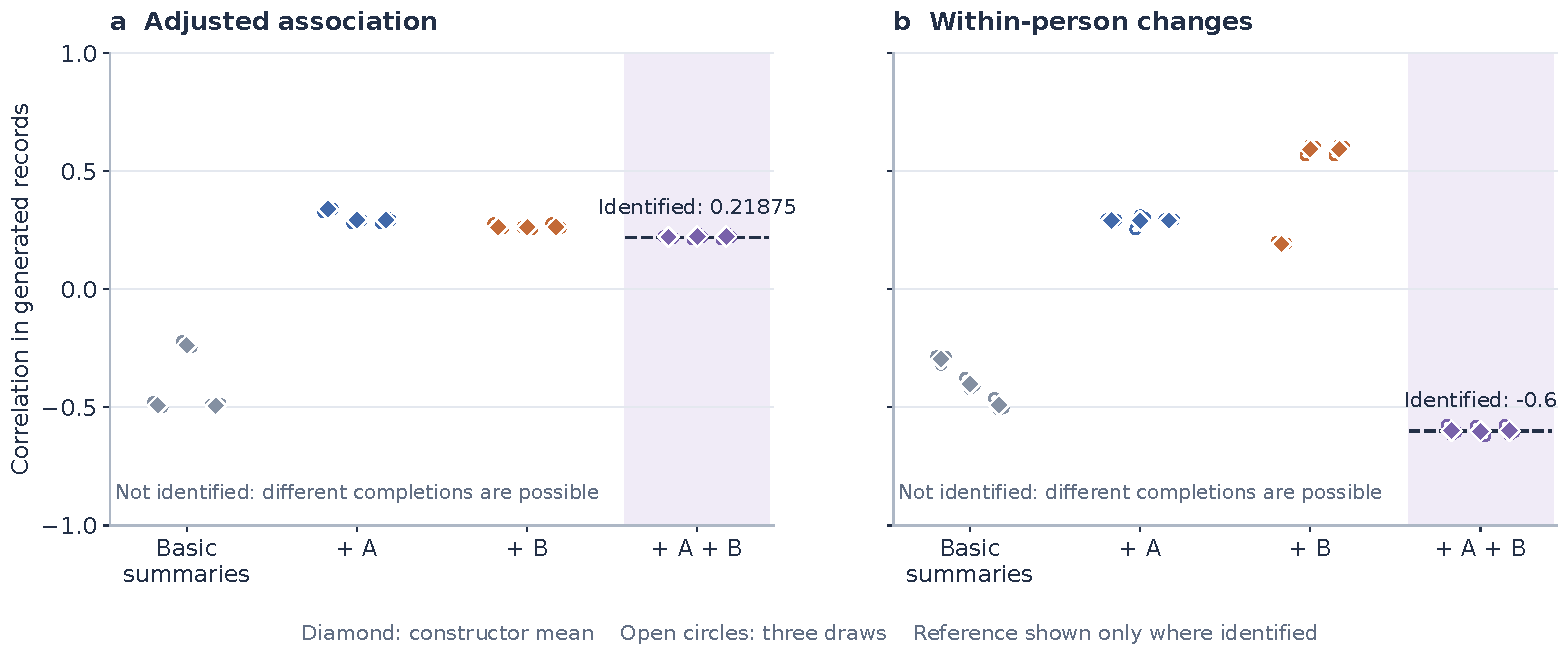
\includegraphics[width=\linewidth]{figures/fig3-evidence-composition.pdf}

\caption{Complementary summaries identify the requested analysis. Diamonds are construction means and open circles/\allowbreak{}ranges are three draws per construction. Panels are artificial mathematical populations, not patient cohorts. The reference is shown only in A+B, where the primary relation is identified. The other cells admit multiple completions and are not ranked by distance from that line. Every one of the 24 constructions is included.}

\label{fig:3}

\end{figure}

\FloatBarrier

\Needspace{5\baselineskip}

\subsection{Joint pressure evidence improves residual dependence beyond extra summaries}

Adding only source context and univariate summaries leaves PNS residual-correlation discrepancy nearly unchanged: BASE 0.16317 and SUMMARY 0.16328. Adding the six joint correlations reduces it to 0.03498, a \textbf{78.6\%} descriptive reduction versus SUMMARY. Every joint-informed construction is closer on this primary endpoint than every summary-only construction in this run. Mean generated correlation changes from 0.5539 to 0.7251, against the existing reference 0.7172. The smaller difference between these last two means is not the MAE; averaging before taking absolute differences would hide construction-level variation.


The Agent records reveal substantive modeling work. All three JOINT constructors independently derive an approximately 0.788 source residual correlation after age/\allowbreak{}BMI projection. Two select a transported innovation correlation of 0.70; the third uses the source conditional covariance with a Student-t innovation construction and support handling. The source projection does not include sex adjustment. These are explicit Agent-selected models and transfer assumptions, not target parameters inserted by the host.


The resulting table is not uniformly closer on all analyses. BMI–\allowbreak{}SBP slope discrepancy increases from 0.3396 to 0.5091 mmHg per 5 kg/\allowbreak{}m², and BMI–\allowbreak{}DBP discrepancy from 0.7378 to 0.7550. All nine constructions retain the older INTERSALT slope anchors. Systolic-pressure SD discrepancy improves from 0.7448 to 0.2991 mmHg; diastolic SD changes little. Figure 4 preserves the complete profile.


\begin{figure}[htbp]

\centering

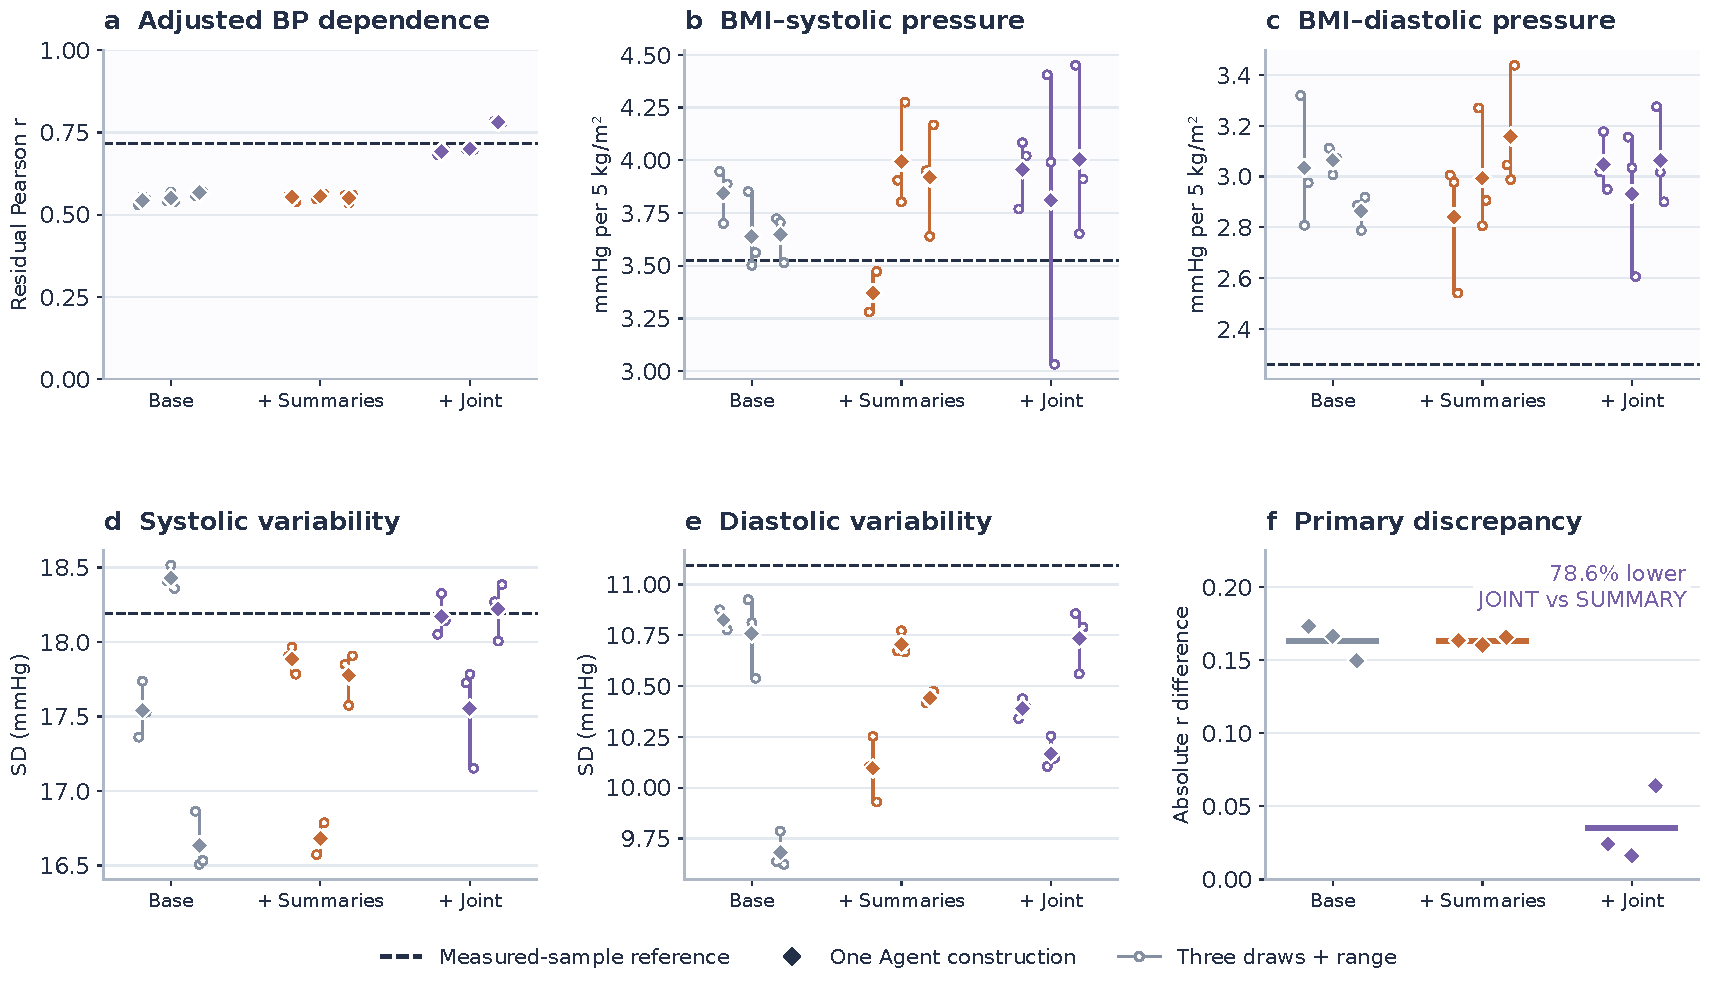
\includegraphics[width=\linewidth]{figures/fig4-pressure-content.pdf}

\caption{Joint information changes the paired-pressure analysis. Panels a–\allowbreak{}c show all three primary analyses and d–\allowbreak{}e both dispersion diagnostics. Gray is BASE, copper adds summaries and purple additionally adds the joint block. Each diamond represents one of three constructions in its condition; small circles/\allowbreak{}ranges show its three draws. Dashed lines are exposed measured-sample point references, not equivalence bands. Panel f compares the primary absolute discrepancy after averaging within each construction; its horizontal bars are arm means. Joint evidence improves residual dependence and systolic dispersion, while both slope discrepancies worsen. The original search episode is reported separately in Figure S1.}

\label{fig:4}

\end{figure}

\FloatBarrier

\Needspace{5\baselineskip}

\subsection{Iron evidence strengthens threshold association but does not identify all continuous uses}

Adding paired iron-status counts moves the generated mean low-marker OR from 3.0638 with marginal summaries to 6.9725. Absolute log-OR discrepancy decreases from 1.7620 to 0.9373, a \textbf{46.8\%} reduction. Every JOINT construction is closer on this endpoint than every SUMMARY construction. Nevertheless, the generated OR remains below the reference 17.7898 (design-based 95\% interval 9.2786–\allowbreak{}34.1083). Improvement is not recovery of that reference.


All three JOINT Agents independently choose a Gaussian copula and numerically solve its latent correlation from the supplied table. The four cells imply source OR 6.6531 and joint prevalence 10.3531\%. Under the selected Gaussian family, a separate source-only calculation gives latent correlation 0.5842 and implied Spearman correlation 0.5661. The host supplied neither a copula nor those derived values. Generated results follow the chosen laws, while different authors select different positive or bounded marginal distributions.


The same evidence addition worsens other requested uses. Joint-prevalence discrepancy increases from 0.5187 to 2.5940 percentage points. Continuous Spearman discrepancy increases from 0.0447 to 0.1736, with generated correlation 0.5720 against 0.3984. The source table constrains binary co-occurrence; it does not identify a continuous copula. The extrapolation from threshold dependence to continuous dependence is an additional modeling assumption.


The provenance record also locates a distinct margin-transport problem. The source has low-ferritin prevalence 504/\allowbreak{}1671 = 30.16\%, versus 12.15\% in the reference sample. Both evidence-augmented arms carry that source margin into generation, producing about 30\%. Low-Hb prevalence, in contrast, remains close to 15\%. These source and target populations differ in selection, geography and measurement conditions; the analysis explains the model-level discrepancy, not the biological cause of the population difference.


\begin{figure}[htbp]

\centering

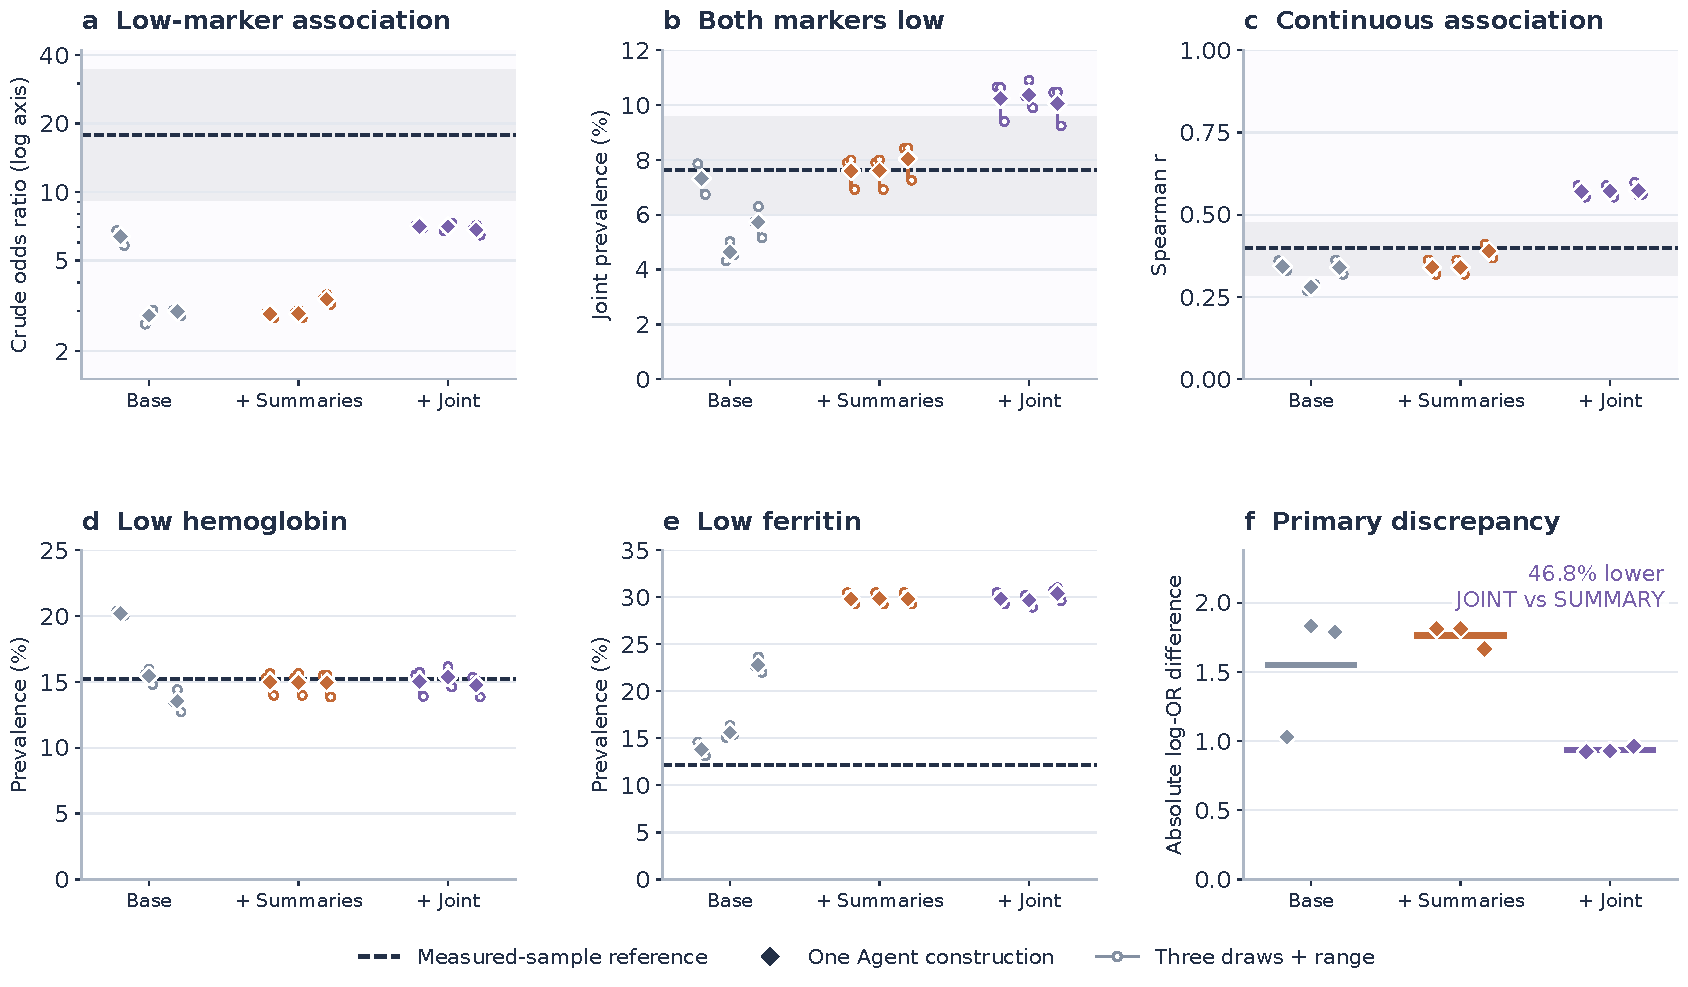
\includegraphics[width=\linewidth]{figures/fig5-iron-content.pdf}

\caption{A better threshold association need not imply a better continuous model. Panels a–\allowbreak{}c show OR, joint prevalence and Spearman correlation; d–\allowbreak{}e show single-marker prevalences. Panel a uses a log axis. Shading in a–\allowbreak{}c shows existing design-based 95\% reference intervals; no intervals are invented for d–\allowbreak{}e. Points and draw ranges use the same construction-level encoding as Figure 4. Panel f shows construction-level absolute log-OR discrepancies and horizontal arm means. JOINT improves this primary comparison, while joint prevalence and rank correlation become less close. Two SUMMARY constructors share the same primary profiles under common seeds; their overlapping results are retained as separate constructions, not counted as extra independent evidence.}

\label{fig:5}

\end{figure}

\FloatBarrier

\Needspace{5\baselineskip}

\Needspace{23\baselineskip}

\subsection{Inspectable decisions connect the evidence to scientific use}

\FloatBarrier

\Needspace{17\baselineskip}

\FloatBarrier

\begingroup

\small

\renewcommand{\arraystretch}{1.22}

\begin{xltabular}{\linewidth}{@{}>{\raggedright\arraybackslash}X>{\raggedright\arraybackslash}X>{\raggedright\arraybackslash}X>{\raggedright\arraybackslash}X@{}}

\caption{What the Agent actually adds between a source and a data table. Derivation and transport remain separate decisions.}\label{tab:3} \\

\toprule

\textbf{Case} & \textbf{Available evidence} & \textbf{Agent decision observed} & \textbf{Consequence and remaining assumption} \\

\midrule

\endfirsthead

\multicolumn{4}{l}{\small Table \thetable\ continued}\\

\toprule

\textbf{Case} & \textbf{Available evidence} & \textbf{Agent decision observed} & \textbf{Consequence and remaining assumption} \\

\midrule

\endhead

\bottomrule

\endfoot

Pressure & Six same-sample correlations, with study context & Projects out age/\allowbreak{}BMI; chooses innovation family and target dependence & Residual analysis improves; sex adjustment and population transfer remain assumed \\

Iron & Four joint-threshold cells plus source margins & Chooses Gaussian copula; solves latent dependence; chooses concentration laws & Threshold OR improves; continuous rank relation is a structural extrapolation \\

Repeated visits & Between-person and same-visit summaries under stipulated structure & Separates stable and visit components; derives change covariance & Negative change relation recovered in the controlled task \\

\end{xltabular}

\endgroup

Mathematical and numerical inspection support these findings. All nine pressure programs and nine iron programs have finite relevant moments under their inspected laws. Final tables show no observed pressure-ordering violations, nonpositive requested biomarker values or duplicate measurement rows under the respective checks. Separate implementations reproduce 162 pressure and 135 iron endpoint values to maximum differences of 8.62 × 10⁻¹⁴ and 8.88 × 10⁻¹⁶. These are computational checks, not independent clinical validations. No submitted scientific law was edited after its results became visible.


Earlier comparisons remain part of the record. A same-model, request-only study found the specialized workflow closer on two of six aggregated analyses and an ordinary Agent closer on four. Later reviews repaired specific mathematical defects, but 66 of 72 tables were unchanged. These findings motivate treating search, checks and revision as available actions rather than claiming that extra scaffolding necessarily improves data quality. Supplement S6 retains the comparison boundaries and unsuccessful source admission.


\Needspace{8\baselineskip}

\section{Discussion}

The data product is feasible and its scientific use can be tested concretely. The lifestyle example demonstrates reusable records for a recognizable adjusted analysis. Controlled tasks demonstrate that an Agent can compose compatible summaries into a relationship that is not supplied directly. Two real-case content controls then show that relevant joint information improves a prespecified joint analysis beyond adding marginal summaries alone. These observations connect the Agent's scientific decisions to an actual data product and its analysis.


The results also clarify the level at which usefulness should be claimed. A virtual table can represent a BMI group contrast while missing a lipid contrast, or better represent a deficiency OR while worsening continuous association. These are different functions of the joint law. The method therefore supports explicit analysis-use statements accompanied by the source-to-model trace. Traceability helps inspect which assumption changed; it is not a calibrated predictor of accuracy or proof that the Agent's self-description is always correct.


Several limits bound the current evidence. The biomedical content controls have three constructions per condition, one current GPT configuration and previously exposed project references. They are fixed-packet tests, not an autonomous-search advantage or a comparison against a neighboring published method. Source admission included coordinator review. Artificial tasks provide exact summaries and stipulated structure, unlike uncertain heterogeneous publications. Recorded usage costs omit investigator effort. Shared seeds and similar model choices can produce closely related outputs across fresh calls.


Most importantly, neither summary consistency nor numerical execution establishes population transport. Sampling intervals around a measured reference do not resolve missing source-to-target assumptions, and repeated virtual samples do not increase the number of observed patients. The current evidence supports scientific-analysis prototyping and reconstruction in the evaluated settings. Claims about replacing clinical measurements, calibrated inferential uncertainty or out-of-population reliability require further validation.


The next experiments should extend a specific claim rather than add generic components. One useful extension is an independently defined biomedical use with an agreed scientific tolerance and an unused evaluation boundary. Another is replication of the same content controls with a second model family. A matched reproduction of a neighboring method can test comparative quality where the task and input regime align. The present results already identify the core method and the evidence-composition question; they do not require turning the paper into a general failure benchmark.


\Needspace{8\baselineskip}

\section{Reproducibility, costs and data-use scope}

This edition integrates closed aggregate results. It runs no new Agent calls, generates no new cohorts and refits no patient data. Frozen protocols, packets, schedules, prompts, requested/\allowbreak{}returned model identifiers, programs and output hashes remain in their original units. All 18 new biomedical constructions and 54 tables are represented. The 216,000 rows in those two experiments are Monte Carlo records from 18 laws, not clinical sample size.


Recorded tariff estimates are USD0.3746075 for lifestyle generation, USD0.6540764 for controlled composition, USD0.9223776 for the pressure content control and USD0.6806303 for the iron content control. The earlier pressure search-plus-generation episode cost USD1.0560459, and the unsuccessful lipid admission cost USD0.7708042. These are stored usage estimates, not invoices or a general price per validated finding.


Patient-level real and virtual records, complete third-party papers and credentials remain local. Shareable materials comprise original code, permitted source metadata, protocols and aggregate results after disclosure review. Applicable dataset conditions govern access and redistribution. The editable manuscript package includes vector figures and LuaLaTeX sources. Author metadata, contribution statements, funding, conflicts, ethics and dataset-specific declarations require completion before submission.


\section*{Supporting materials and reproducibility}

The supplement retains all numerical profiles, exact controlled derivations, the earlier search episode and historical comparison boundaries. The unchanged expanded v0.31 remains the full developmental record; v0.32 is preserved as the previous focused edition. This integration supplies a protected-input manifest, plotted-value ledger, claim-to-evidence map and PDF/\allowbreak{}build audit.


\clearpage

\section*{References}

\begingroup

\begin{enumerate}[label=\arabic*.,leftmargin=2.1em,itemsep=.2em,parsep=0pt]

\item Holt S, Ruiz Luyten M, Berthon A, van der Schaar M. G-Sim: Generative Simulations with Large Language Models and Gradient-Free Calibration. \emph{Proceedings of ICML}. PMLR 267;2025:23513–\allowbreak{}23561. \href{https://proceedings.mlr.press/v267/holt25b.html}{Published record}.

\item Tang Y, Kong M, He J, Nie T, Ma W, Sun L. LLMSynthor: Macro-Aligned Micro-Records Synthesis with Large Language Models. KDD 2026. \href{https://doi.org/10.1145/3770855.3818965}{DOI}; \href{https://arxiv.org/html/2505.14752v4}{full text v4}.

\item Filshtein TJ, Li X, Zimmerman SC, Ackley SF, Glymour MM, Power MC. Proof of concept example for use of simulation to allow data pooling despite privacy restrictions. \emph{Epidemiology}. 2021;32(5):638–\allowbreak{}647. \href{https://pmc.ncbi.nlm.nih.gov/articles/PMC8338788/}{DOI and full text}.

\item Zhao Z et al. SynthIPD: training-free synthetic individual patient data generation. arXiv:2509.16466v2, 24 July 2026. \href{https://arxiv.org/html/2509.16466v2}{Versioned full text}. Publication beyond this preprint was not established in the positioning audit.

\item Jiang J, Gao C, Rasmussen E, Xie SZ, Sun J. KMGen: A Skill-based Approach for Synthetic Individual Patient Data Generation. MLHC 2026, PMLR 340:755–\allowbreak{}814. \href{https://proceedings.mlr.press/v340/jiang26a.html}{Official proceedings}.

\item Callender T, Boyd A, Davis R, Ruhrberg Estevez S, Lavista Ferres JM, van der Schaar M. SynthCraft: An AI partner for synthetic data generation to support data access and augmentation in healthcare. \emph{PLOS Digital Health}. 2026;5(3):e0001290. \href{https://journals.plos.org/digitalhealth/article?id=10.1371/journal.pdig.0001290}{Published article}.

\item Phillippo DM et al. Multilevel network meta-regression for population-adjusted treatment comparisons. \emph{Journal of the Royal Statistical Society: Series A}. 2020;183(3):1189–\allowbreak{}1210. \href{https://rss.onlinelibrary.wiley.com/doi/full/10.1111/rssa.12579}{DOI/\allowbreak{}full text}.

\item Gu T, Taylor JMG, Mukherjee B. A synthetic data integration framework to leverage external summary-level information from heterogeneous populations. \emph{Biometrics}. 2023;79:3831–\allowbreak{}3845. \href{https://doi.org/10.1111/biom.13852}{DOI}.

\item Lea AJ, Martins D, Kamau J, Gurven M, Ayroles JF. Urbanization and market integration have strong, nonlinear effects on cardiometabolic health in the Turkana. \emph{Science Advances}. 2020;6:eabb1430. \href{https://doi.org/10.1126/sciadv.abb1430}{Article}. \href{https://doi.org/10.5061/dryad.2z34tmpjk}{Dataset}.

\item Pesquisa Nacional de Saúde. PNS 2013 public survey and laboratory data. \href{https://www.pns.icict.fiocruz.br/bases-de-dados/}{Survey files}; \href{https://www.pns.icict.fiocruz.br/exames-laboratoriais/}{laboratory information}.

\item Jaspert FM, Harling G, Sie A, Bountogo M, Bärnighausen T, Ditzen B, Fischer MS. Association of relationship satisfaction with blood pressure: a cross-sectional study of older adults in rural Burkina Faso. BMJ Open. 2024;14:e089374. \href{https://doi.org/10.1136/bmjopen-2024-089374}{Original article}.

\item Aheto JMK, Gates T, Babah R, Takramah W. Joint modelling of systolic and diastolic blood pressure and its associated factors among women in Ghana: Multivariate response multilevel modelling methods. PLOS Global Public Health. 2023;3:e0001613. \href{https://pmc.ncbi.nlm.nih.gov/articles/PMC10132648/}{Original article}.

\item Zhu JH et al. Iron, Folate, and B12 Deficiencies and their Associations with Anemia among Women of Childbearing Age in a Rural Area in Northern China. \emph{International Journal for Vitamin and Nutrition Research}. 2010;80(2):144–\allowbreak{}154. \href{https://doi.org/10.1024/0300-9831/a000014}{DOI}. Original Tables I and IV provide the admitted iron evidence.

\item National Center for Health Statistics. NHANES August 2021–\allowbreak{}August 2023 laboratory documentation. \href{https://wwwn.cdc.gov/Nchs/Data/Nhanes/Public/2021/DataFiles/FERTIN\_L.htm}{Ferritin, FERTIN\_L}; \href{https://wwwn.cdc.gov/Nchs/Data/Nhanes/Public/2021/DataFiles/CBC\_L.htm}{Complete blood count, CBC\_L}. Published September 2024; documentation checked 17 November 2026.

\end{enumerate}

\endgroup

\clearpage

\appendix

\section*{Supplementary results}

\setcounter{figure}{0}

\renewcommand{\thefigure}{S\arabic{figure}}

\renewcommand{\theHfigure}{S\arabic{figure}}

\setcounter{table}{0}

\renewcommand{\thetable}{S\arabic{table}}

\renewcommand{\theHtable}{S\arabic{table}}

\FloatBarrier

\Needspace{5\baselineskip}

\subsection*{S1. Complete lifestyle profile and analysis boundary}

Table S1 gives all nine primary raw-scale contrasts with both constructions, rather than filtering by the direction or size of agreement. The interval is the conventional model-based interval from the measured-sample analysis. Author means average three prespecified draws; they are not pooled patient observations. Standardizing each biomarker within each dataset changes the numerical scale, so raw effects remain primary for this comparison.


\FloatBarrier

\begingroup

\small

\renewcommand{\arraystretch}{1.22}

\begin{xltabular}{\linewidth}{@{}>{\raggedright\arraybackslash}X>{\raggedright\arraybackslash}X>{\raggedright\arraybackslash}X>{\raggedright\arraybackslash}X@{}}

\caption{All primary lifestyle contrasts. Author values are means across three virtual draws; real intervals are 95\% model-based intervals. BMI is in kg/\allowbreak{}m² and both cholesterol measures are in mg/\allowbreak{}dL.}\label{tab:4} \\

\toprule

\textbf{Trait and contrast} & \textbf{Real estimate [95\% interval]} & \textbf{Agent 1} & \textbf{Agent 2} \\

\midrule

\endfirsthead

\multicolumn{4}{l}{\small Table \thetable\ continued}\\

\toprule

\textbf{Trait and contrast} & \textbf{Real estimate [95\% interval]} & \textbf{Agent 1} & \textbf{Agent 2} \\

\midrule

\endhead

\bottomrule

\endfoot

BMI: urban − pastoralist & 1.882 [1.368, 2.397] & 2.047 & 1.972 \\

BMI: urban − rural & 1.640 [1.227, 2.053] & 1.918 & 1.811 \\

BMI: rural − pastoralist & 0.242 [-0.172, 0.656] & 0.129 & 0.161 \\

Total cholesterol: urban − pastoralist & 20.342 [4.467, 36.217] & 14.959 & 16.535 \\

Total cholesterol: urban − rural & 10.849 [-3.313, 25.011] & 13.902 & 15.667 \\

Total cholesterol: rural − pastoralist & 9.493 [-0.373, 19.359] & 1.058 & 0.868 \\

HDL: urban − pastoralist & 1.750 [-5.474, 8.975] & -0.091 & -0.447 \\

HDL: urban − rural & -2.696 [-9.147, 3.755] & 0.679 & 0.460 \\

HDL: rural − pastoralist & 4.446 [-0.062, 8.954] & -0.770 & -0.908 \\

\end{xltabular}

\endgroup

The real pool used age greater than 18, with nine otherwise available 18-year-olds excluded. No generated row was affected by that boundary in this unit. Biomarker-specific complete-case availability differs substantially between real and virtual tables. The full analysis retained 189 group-contrast estimates and 21 interaction tests across the seven datasets, including the measured reference. The plotted primary subset contains nine contrasts per dataset. A separate numerical implementation made 4,690 comparisons, with maximum difference 8.52 × 10⁻¹³. These are computational checks, not 4,690 scientific validations.


Original records: \texttt{work/\allowbreak{}lifestyle\_\allowbreak{}application\_\allowbreak{}2026-\allowbreak{}11-\allowbreak{}11/\allowbreak{}RESULTS.md} and \texttt{ANALYSIS\_\allowbreak{}CONTRASTS.csv}. All sex-specific outputs, diagnostics, full laws and author records remain in that completed unit. The use of the original publication's conclusions is intentional and is not an independent-reference design.


\FloatBarrier

\Needspace{5\baselineskip}

\subsection*{S2. What the composition tasks identify}

In the adjusted task, all variables have mean zero and variance one. A reports marginal correlation \(r_{XY}=0.5\); B reports \(r_{XZ}=r_{YZ}=0.6\). The correlation of linear-projection residuals is


\[
r_{XY\cdot Z}=\frac{r_{XY}-r_{XZ}r_{YZ}}{\sqrt{(1-r_{XZ}^{2})(1-r_{YZ}^{2})}}=\frac{0.5-0.36}{0.64}=0.21875.
\]

This identity describes linear residual correlation, not arbitrary conditional independence. It does not require a Gaussian population. The Agents chose Gaussian generators, but the evaluator did not require that family. A alone identifies marginal X–\allowbreak{}Y correlation, B alone identifies the X-on-Z slope, and both identify the primary residual correlation. Basic-only, A-only and B-only do not identify that primary quantity.


In the longitudinal task, each visit is a stable person component plus a mean-zero deviation. Stable-component variances are 4, visit-deviation variances are 1, the two components are independent, and deviations at different visits are independent. These assumptions are supplied in every condition. A gives a between-person correlation of 0.8, so the stable covariance is 3.2. B gives a same-visit correlation of 0.52, so total same-visit covariance is 2.6. The within-visit deviation covariance must therefore be −0.6. With independent visit deviations, the covariance of changes is twice that quantity and each change variance is 2, yielding change correlation −0.6. Cross-visit correlation is 3.2/\allowbreak{}5 = 0.64. The negative change relation can coexist with a positive same-visit relation under the stipulated structure.


\FloatBarrier

\begingroup

\small

\renewcommand{\arraystretch}{1.22}

\begin{xltabular}{\linewidth}{@{}>{\hsize=1.350000\hsize\linewidth=\hsize\raggedright\arraybackslash}X>{\hsize=0.912500\hsize\linewidth=\hsize\raggedright\arraybackslash}X>{\hsize=0.912500\hsize\linewidth=\hsize\raggedright\arraybackslash}X>{\hsize=0.912500\hsize\linewidth=\hsize\raggedright\arraybackslash}X>{\hsize=0.912500\hsize\linewidth=\hsize\raggedright\arraybackslash}X@{}}

\caption{Complete controlled primary results. Each row has three fresh constructions and nine draws. Ranges describe the three construction means. Error is scored only when the primary relation is identified.}\label{tab:5} \\

\toprule

\textbf{Task} & \textbf{Evidence} & \textbf{Primary range} & \textbf{Primary MAE} & \textbf{Source checks} \\

\midrule

\endfirsthead

\multicolumn{5}{l}{\small Table \thetable\ continued}\\

\toprule

\textbf{Task} & \textbf{Evidence} & \textbf{Primary range} & \textbf{Primary MAE} & \textbf{Source checks} \\

\midrule

\endhead

\bottomrule

\endfoot

Adjusted & Basic & -0.4930 to -0.2380 & Not identified & 54/\allowbreak{}54 \\

Adjusted & Basic + A & 0.2926 to 0.3387 & Not identified & 63/\allowbreak{}63 \\

Adjusted & Basic + B & 0.2615 to 0.2624 & Not identified & 72/\allowbreak{}72 \\

Adjusted & Basic + A + B & 0.2211 to 0.2230 & 0.00731 & 81/\allowbreak{}81 \\

Longitudinal & Basic & -0.4911 to -0.2966 & Not identified & 108/\allowbreak{}108 \\

Longitudinal & Basic + A & 0.2893 to 0.2907 & Not identified & 117/\allowbreak{}117 \\

Longitudinal & Basic + B & 0.1911 to 0.5923 & Not identified & 117/\allowbreak{}117 \\

Longitudinal & Basic + A + B & -0.6013 to -0.5991 & 0.01492 & 126/\allowbreak{}126 \\

\end{xltabular}

\endgroup

All 90 identified estimates include primary and secondary functionals across conditions. There are 18 primary estimates in combined cells, not 90 independent primary tests. The full 216 estimates, identification labels, source-check details and failures are retained. There were no construction or execution failures in the 24-slot unit. The three seeds were 16101, 16103 and 16109. The 57 unique numeric tables among 72 outputs do not change the construction denominator.


The original records remain in the frozen composition unit. Its protocol and bindings are in \texttt{PROTOCOL.md} and \texttt{FREEZE.json}; its analysis directory contains \texttt{analyses.csv}, \texttt{constructor\_\allowbreak{}analyses.csv} and \texttt{INDEPENDENT\_\allowbreak{}RECOMPUTATION.json}.


\FloatBarrier

\Needspace{5\baselineskip}

\subsection*{S3. Pressure content control}

\FloatBarrier

\begingroup

\small

\renewcommand{\arraystretch}{1.22}

\begin{xltabular}{\linewidth}{@{}>{\hsize=1.350000\hsize\linewidth=\hsize\raggedright\arraybackslash}X>{\hsize=0.912500\hsize\linewidth=\hsize\raggedright\arraybackslash}X>{\hsize=0.912500\hsize\linewidth=\hsize\raggedright\arraybackslash}X>{\hsize=0.912500\hsize\linewidth=\hsize\raggedright\arraybackslash}X>{\hsize=0.912500\hsize\linewidth=\hsize\raggedright\arraybackslash}X@{}}

\caption{Complete pns profile. Entries are mean estimate / mean absolute discrepancy. Absolute differences are computed before construction and arm averaging.}\label{tab:6} \\

\toprule

\textbf{Analysis} & \textbf{Sample reference} & \textbf{BASE} & \textbf{SUMMARY} & \textbf{JOINT} \\

\midrule

\endfirsthead

\multicolumn{5}{l}{\small Table \thetable\ continued}\\

\toprule

\textbf{Analysis} & \textbf{Sample reference} & \textbf{BASE} & \textbf{SUMMARY} & \textbf{JOINT} \\

\midrule

\endhead

\bottomrule

\endfoot

Residual Pearson r & 0.7172 & 0.5540 / 0.1632 & 0.5539 / 0.1633 & 0.7251 / 0.0350 \\

BMI–\allowbreak{}SBP (mmHg/\allowbreak{}5 kg/\allowbreak{}m²) & 3.5240 & 3.7103 / 0.1934 & 3.7617 / 0.3396 & 3.9238 / 0.5091 \\

BMI–\allowbreak{}DBP (mmHg/\allowbreak{}5 kg/\allowbreak{}m²) & 2.2599 & 2.9875 / 0.7276 & 2.9977 / 0.7378 & 3.0149 / 0.7550 \\

SBP SD (mmHg) & 18.1916 & 17.5350 / 0.8140 & 17.4468 / 0.7448 & 17.9824 / 0.2991 \\

DBP SD (mmHg) & 11.0941 & 10.4221 / 0.6721 & 10.4139 / 0.6803 & 10.4312 / 0.6630 \\

\end{xltabular}

\endgroup

The two augmented arms share the Burkina Faso population description and univariate summaries. Its admitted matrix describes 2,114 complete-case partnered adults aged at least 40, excluding recent antihypertensive use and pregnancy, with pressure averaged from the last two of three seated measurements. Source age/\allowbreak{}BMI projection does not identify sex-adjusted target dependence. The original BASE packet retains its historical extraction status; this unit did not reauthenticate every old source. Source uncertainty, rounding and transport are not converted into fabricated target intervals.


All nine models are sampled at seeds 16211, 16213 and 16217. The programs are sealed before 27 final outputs and aggregate comparison. Every table has a unique hash. The pressure-ordering violation fraction is zero for every draw, the sixth endpoint in the independent 162-value calculation. Case-specific source audit, model decisions, receipts and full outputs remain in \texttt{work/\allowbreak{}pns\_\allowbreak{}evidence\_\allowbreak{}content\_\allowbreak{}control\_\allowbreak{}2026-\allowbreak{}11-\allowbreak{}16}. Figure 4 plots all five scientific metrics rather than only the primary gain.


\FloatBarrier

\Needspace{5\baselineskip}

\subsection*{S4. Iron content control}

\FloatBarrier

\begingroup

\small

\renewcommand{\arraystretch}{1.22}

\begin{xltabular}{\linewidth}{@{}>{\hsize=1.350000\hsize\linewidth=\hsize\raggedright\arraybackslash}X>{\hsize=0.912500\hsize\linewidth=\hsize\raggedright\arraybackslash}X>{\hsize=0.912500\hsize\linewidth=\hsize\raggedright\arraybackslash}X>{\hsize=0.912500\hsize\linewidth=\hsize\raggedright\arraybackslash}X>{\hsize=0.912500\hsize\linewidth=\hsize\raggedright\arraybackslash}X@{}}

\caption{Complete iron profile. Entries are mean estimate / mean absolute discrepancy. Absolute differences are computed before construction and arm averaging.}\label{tab:7} \\

\toprule

\textbf{Analysis} & \textbf{Sample reference} & \textbf{BASE} & \textbf{SUMMARY} & \textbf{JOINT} \\

\midrule

\endfirsthead

\multicolumn{5}{l}{\small Table \thetable\ continued}\\

\toprule

\textbf{Analysis} & \textbf{Sample reference} & \textbf{BASE} & \textbf{SUMMARY} & \textbf{JOINT} \\

\midrule

\endhead

\bottomrule

\endfoot

Crude OR / absolute log-OR difference & 17.7898 & 4.0659 / 1.5495 & 3.0638 / 1.7620 & 6.9725 / 0.9373 \\

Both low (\%) / pp difference & 7.6304 & 5.8911 / 1.7903 & 7.7511 / 0.5187 & 10.2244 / 2.5940 \\

Continuous Spearman r & 0.3984 & 0.3215 / 0.0769 & 0.3564 / 0.0447 & 0.5720 / 0.1736 \\

Low Hb (\%) / pp difference & 15.2401 & 16.3978 / 2.3844 & 14.9711 / 0.5978 & 15.0644 / 0.6022 \\

Low ferritin (\%) / pp difference & 12.1531 & 17.4289 / 5.2758 & 29.8400 / 17.6869 & 29.9844 / 17.8314 \\

\end{xltabular}

\endgroup

The source four-cell table is both low 173, Hb-only 85, ferritin-only 331 and neither low 1,082, after collapsing the folate/\allowbreak{}B12 categories. The source crude OR is 6.6531. It must not be confused with the paper's separately adjusted OR of 6.4. Agents saw the source cells and definitions, not these derived ORs or a prescribed copula. The source population includes selected parous rural Chinese women, 2–\allowbreak{}4 years postpartum and using IUD contraception; it is not a representative US target sample.


The existing NHANES reference uses a stratified delete-one-PSU JKn calculation, with 15 strata, 30 PSUs and 15 degrees of freedom. Its 95\% intervals are OR 9.2786–\allowbreak{}34.1083, joint prevalence 6.0681–\allowbreak{}9.5541\% and Spearman 0.3183–\allowbreak{}0.4729. No intervals were calculated for the two displayed marginal fractions in this unit. The stored weighted reference is parsed after the new construction and generation outputs close. The project had already seen it historically; delayed parsing does not make it a new holdout.


All nine laws have finite relevant moments. Five bound both concentrations; one has ideal half-normal log tails with finite positive polynomial moments and an additional numerical probability guard; three have bounded Hb and positive lognormal-type ferritin tails. No post-submission scientific edits are made. One provenance classification remains incorrect: BASE\_2 labels its source-suitability assessment REPORTED although it is an Agent assessment. Origin records therefore remain inspectable evidence, not infallible truth labels.


All 27 tables have distinct hashes. SUMMARY\_1 and SUMMARY\_2 nevertheless have identical three-seed primary profiles because their threshold probabilities, latent dependence and common seeds coincide; there are 24 unique primary draw triplets. No construction is removed or counted as an independent scientific replication merely because its rows differ. Seeds are 16311, 16313 and 16317. All 135 scientific endpoints independently agree to 8.88 × 10⁻¹⁶. Full records remain in \texttt{work/\allowbreak{}iron\_\allowbreak{}evidence\_\allowbreak{}content\_\allowbreak{}control\_\allowbreak{}2026-\allowbreak{}11-\allowbreak{}16}.


\FloatBarrier

\Needspace{5\baselineskip}

\subsection*{S5. Earlier search-to-generation pressure episode}

Before the three-condition control, an API-connected search Agent made 14 queries and retrieved six full texts. Coordinator original-source review admitted Burkina Faso and Ghana records [11,12]. Six fresh constructors received original or augmented packets, producing 18 tables. The mean residual correlation moved from 0.5376 to 0.7046; MAE fell from 0.17962 to 0.01277 (92.89\%). This favorable exploratory result motivated the content-control experiment; it is not the latter's effect estimate. The new 78.6\% result uses different fresh constructions and a more specific SUMMARY comparison.


\begin{figure}[htbp]

\centering

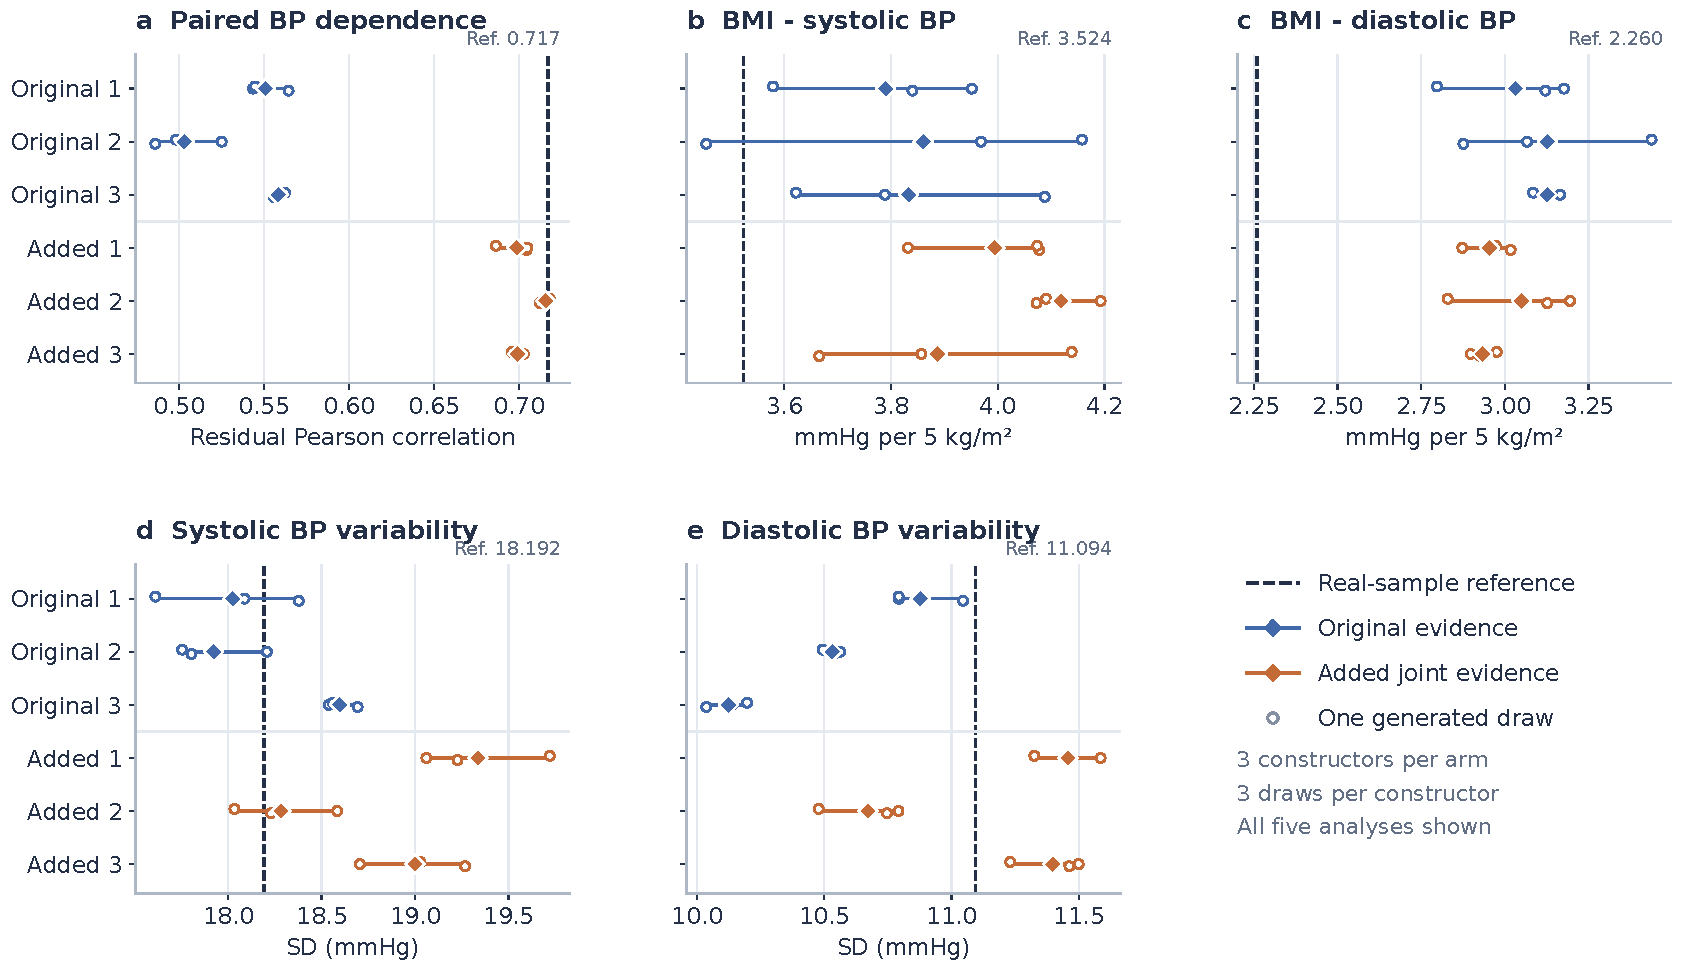
\includegraphics[width=\linewidth]{figures/figS1-search-followup.pdf}

\caption{Earlier search follow-up, kept distinct from the new content control. All three primary analyses and two scale diagnostics are shown for three constructions per arm, each sampled three times. Points, draw ranges and reference lines have the same interpretation as Figure 4. Added evidence improves residual dependence and diastolic outcomes while worsening systolic slope and spread agreement. This episode changes the entire source packet and does not isolate the effect of its joint statistics.}

\label{fig:6}

\end{figure}

\FloatBarrier

\Needspace{17\baselineskip}

\FloatBarrier

\begingroup

\small

\renewcommand{\arraystretch}{1.22}

\begin{xltabular}{\linewidth}{@{}>{\hsize=1.350000\hsize\linewidth=\hsize\raggedright\arraybackslash}X>{\hsize=0.912500\hsize\linewidth=\hsize\raggedright\arraybackslash}X>{\hsize=0.912500\hsize\linewidth=\hsize\raggedright\arraybackslash}X>{\hsize=0.912500\hsize\linewidth=\hsize\raggedright\arraybackslash}X>{\hsize=0.912500\hsize\linewidth=\hsize\raggedright\arraybackslash}X@{}}

\caption{Blood-pressure analysis and dispersion results. Each condition has three constructions and nine draws. Mean absolute difference is averaged within constructions and then across constructions; the reference is an exposed sample estimate.}\label{tab:8} \\

\toprule

\textbf{Analysis} & \textbf{Reference} & \textbf{Original mean} & \textbf{Added mean} & \textbf{Original / added MAE} \\

\midrule

\endfirsthead

\multicolumn{5}{l}{\small Table \thetable\ continued}\\

\toprule

\textbf{Analysis} & \textbf{Reference} & \textbf{Original mean} & \textbf{Added mean} & \textbf{Original / added MAE} \\

\midrule

\endhead

\bottomrule

\endfoot

Residual correlation & 0.7172 & 0.5376 & 0.7046 & 0.17962 / 0.01277 \\

BMI–\allowbreak{}SBP (mmHg/\allowbreak{}5 kg/\allowbreak{}m²) & 3.5240 & 3.8280 & 4.0001 & 0.31944 / 0.47613 \\

BMI–\allowbreak{}DBP (mmHg/\allowbreak{}5 kg/\allowbreak{}m²) & 2.2599 & 3.0951 & 2.9795 & 0.83516 / 0.71955 \\

SBP SD (mmHg) & 18.1916 & 18.1816 & 18.8729 & 0.32525 / 0.71631 \\

DBP SD (mmHg) & 11.0941 & 10.5107 & 11.1757 & 0.58344 / 0.36284 \\

\end{xltabular}

\endgroup

The added evidence was selected for its statistical content before evaluating the newly generated outputs. Source admission was not based on choosing a statistic close to the PNS estimate. Nevertheless, the target family and its earlier estimates were historically known to the project, so this remains developmental evidence. The new author contexts did not receive those estimates, prior outputs or desired target signs. The original packet was reused with its historical extraction status; this unit did not reauthenticate every old source.


Burkina Faso reports a complete-case sample of 2,114 partnered adults aged at least 40, excluding recent antihypertensive use and pregnancy. Pressure is the average of the last two of three seated measurements. The source age/\allowbreak{}BMI covariance projection does not provide sex adjustment. Ghana analyzes women aged 15–\allowbreak{}49 with categorical age, binary obesity and additional covariates. Its individual residual variances are 224.49 and 101.75 mmHg² with correlation 0.73; household variances are 38.91 and 16.37 mmHg² with correlation 0.81. Correlations cannot be combined without the variance components and the intended estimand. Neither article supplies a transferable uncertainty interval for the target relation.


The Ghana report contains an individual-level column labeled “Child,” despite the methods specifying women, and inconsistent household counts. These issues were recorded; they were not silently corrected into invented precision. A third candidate from Uganda was withheld because 0.7307 was described ambiguously as both an outcome and residual correlation, under a different adjustment set. No source-level replay under these three studies' complete populations was demonstrated. Generated target diagnostics are not relabeled as source replay.


All final draws used seeds 16121, 16123 and 16127. The selected programs and all outputs closed before aggregate comparison. Original records: \texttt{work/\allowbreak{}pns\_\allowbreak{}joint\_\allowbreak{}evidence\_\allowbreak{}2026-\allowbreak{}11-\allowbreak{}16/\allowbreak{}PROTOCOL.md}, \texttt{SOURCE\_\allowbreak{}AUDIT.md}, \texttt{IMPLEMENTATION\_\allowbreak{}REVIEW.md}, \texttt{analysis/\allowbreak{}author\_\allowbreak{}results.json} and \texttt{analysis/\allowbreak{}REFERENCE\_\allowbreak{}USED.json}.


\FloatBarrier

\Needspace{5\baselineskip}

\Needspace{23\baselineskip}

\subsection*{S6. Historical checks, unsuccessful admission and replay boundaries}

\FloatBarrier

\begingroup

\small

\renewcommand{\arraystretch}{1.22}

\begin{xltabular}{\linewidth}{@{}>{\raggedright\arraybackslash}X>{\raggedright\arraybackslash}X>{\raggedright\arraybackslash}X@{}}

\caption{Historical evidence retained alongside the main studies. These are separate developmental experiments, not a common frozen benchmark.}\label{tab:9} \\

\toprule

\textbf{Evidence block} & \textbf{Retained finding} & \textbf{Interpretation} \\

\midrule

\endfirsthead

\multicolumn{3}{l}{\small Table \thetable\ continued}\\

\toprule

\textbf{Evidence block} & \textbf{Retained finding} & \textbf{Interpretation} \\

\midrule

\endhead

\bottomrule

\endfoot

Glycemia & Conditional BMI and residual spread do not uniformly improve & Different historical packets and exposed references \\

Earlier iron study & Threshold summaries are representable; transfer differs & Two constructions; separate from the new content control \\

Repeated follow-up & Rich model exports support requested analyses & Information-rich reconstruction \\

Ordinary Agent versus workflow & Workflow closer on 2/\allowbreak{}6 aggregate analyses & 12 constructions; no consistent superiority \\

Paired review & Tail and rounding repairs; 66/\allowbreak{}72 tables unchanged & 24 dependent review sessions \\

New lipid search & No complete admissible increment packet & No new construction or table \\

\end{xltabular}

\endgroup

The lipid follow-up is particularly important to interpret correctly. Its search Agent made 16 searches and retrieved seven original articles, but exhausted the input budget without completing its report. One documented source-only synthesis attempt also reached its output limit. Original-paper review retained partial constraints and unresolved operator or common-row issues. The contingent nine constructions and 27 tables were not launched. The result is an admission and execution limitation, not evidence that joint literature is absent or that a generated lipid model failed.


One useful control-design lesson emerged: the variance of non-HDL cholesterol, together with total-cholesterol and HDL variances from the same rows, determines their raw covariance. A control that removes an explicit correlation field but retains those three variances has not removed joint information. Reporting precision and shared-row assumptions must also be carried through that derivation. This lesson informs evidence accounting; it is not an additional successful biomedical experiment.


The paired scientific-review programs repaired a divergent tail and a possible threshold-rounding failure, while 66/\allowbreak{}72 final tables remained byte-identical. Finite observed values do not prove a finite population mean; mathematical review and scientific accuracy are distinct. These older repairs are documented in the unchanged expanded manuscript and \texttt{work/\allowbreak{}scientific\_\allowbreak{}check\_\allowbreak{}revision\_\allowbreak{}2026-\allowbreak{}11-\allowbreak{}11/\allowbreak{}RESULTS.md}. They are not credited as gains from the one-call content controls.


Reproduction has three levels: plotting released aggregates; resampling a frozen law under its recorded environment and access conditions; and initiating a new API construction using recorded prompts and tools. The last is stochastic and model availability can change. Earlier host-mediated episodes with incomplete backend identifiers are not described as fully recorded API runs. The controlled and content-control units retain explicit requested/\allowbreak{}returned IDs and usage. Independent numerical recomputation here means a separate implementation within the same research process, not an external investigator's adjudication.

\end{document}
